\documentclass[../../../../main.tex]{subfiles}

\begin{document}

\section*{第1問}

[解] 題意の円を $C$ とおく。
\[ C \equiv (x-2)^2+(y+1)^2=4 \]
から, $O(2, -1), \, r=2$ である。そこで,
\[ \vec{OP} = \begin{pmatrix} x-2 \\ y+1 \end{pmatrix} \]
だから, $\vec{OQ} = k\vec{OP} \quad (k>0)$ とおけることより,
\[ |\vec{OP}| \cdot |\vec{OQ}| = k \{ (x-2)^2+(y+1)^2 \} = 4 \quad (\because \text{題意}) \]
$O \ne P$ から
\[ k = \frac{4}{(x-2)^2+(y+1)^2} \]
だから,
\[ \vec{OQ} = \begin{pmatrix} X-2 \\ Y+1 \end{pmatrix} = \frac{4}{(x-2)^2+(y+1)^2} \begin{pmatrix} x-2 \\ y+1 \end{pmatrix} \]
である。成分を比較して
\[
\begin{cases}
X = \dfrac{4(x-2)}{(x-2)^2+(y+1)^2} + 2 \\[10pt]
Y = \dfrac{4(y+1)}{(x-2)^2+(y+1)^2} - 1
\end{cases}
\quad \text{/\mkern-6mu/ (1)}
\]

(2) $x \in \mathbb{R}, \, y=0$ だから, (1) より
\[
\begin{cases}
X-2 = \dfrac{4(x-2)}{(x-2)^2+1} \\[10pt]
Y+1 = \dfrac{4}{(x-2)^2+1}
\end{cases}
\quad \dots (*)
\]
$Y \ne -1$ だから (第2式より), 第2式を変形して,
\[ (x-2)^2+1 = \frac{4}{Y+1} \]
第1式に代入して,
\[ X-2 = (Y+1)(x-2) \]
\[ \therefore x-2 = \frac{X-2}{Y+1} \quad (\because Y \ne -1) \]
だから, $(*)$ に代入して
\[ Y+1 = \frac{4}{\left( \dfrac{X-2}{Y+1} \right)^2 + 1} \]
\[ \therefore (X-2)^2 + (Y+1)^2 = 4(Y+1) \quad (\because Y \ne -1) \]
\[ (X-2)^2 + (Y-1)^2 = 4 \quad \dots \text{①} \]
又, $(*)$ 及び $x \in \mathbb{R}$ から,
\[ 0 < Y+1 \le 4 \quad \therefore -1 < Y \le 3 \]
に注意して, $(X, Y) \ne (2, -1)$ である。以上から
\[ (X-2)^2 + (Y-1)^2 = 4 \quad ((X, Y)=(2, -1) \text{を除く}) _{\mathbin{/\mkern-6mu/}} \]

\begin{center}
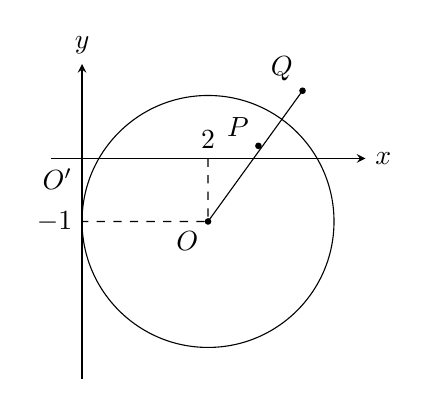
\begin{tikzpicture}[scale=0.8, >=stealth]
  \draw[->] (-0.5,0) -- (4.5,0) node[right] {$x$};
  \draw[->] (0,-3.5) -- (0,1.5) node[above] {$y$};
  \node[below left] at (0,0) {$O'$};
  \coordinate (O) at (2,-1);
  \draw[dashed] (2,0) node[above] {$2$} -- (O) -- (0,-1) node[left] {$-1$};
  \draw (O) circle (2);
  \fill (O) circle (1.5pt) node[below left] {$O$};
  \coordinate (P) at (2.8,0.2);
  \coordinate (Q) at (3.5,1.075);
  \draw (O) -- (Q);
  \fill (P) circle (1.5pt) node[above left] {$P$};
  \fill (Q) circle (1.5pt) node[above left] {$Q$};
\end{tikzpicture}
\end{center}

\section*{第2問}

[解] 判別式として $D > 0 \iff p^2 - 2q > 0 \quad \dots \text{①}$ である。又, 収束する条件から
\[ -1 < \frac{\alpha}{2\beta} \le 1, \quad -1 < \frac{4\beta^2}{\alpha} \le 1 \quad \dots \text{②} \]
ここで, ①の $p > 1 \land 1-2p+2q \ge 0$ を図示すると右図斜線部 (境界は実線のみ含む) だから, $p, q > 0$ となり
\[ \alpha + \beta = p > 0, \quad \alpha\beta = \frac{q}{2} > 0 \quad \dots \text{③} \]
から $\alpha > 0, \, \beta > 0$ である。したがって, ②から
\[ -2\beta < \alpha \le 2\beta, \quad -\alpha < 4\beta^2 \le \alpha \]
\[ \therefore 0 < \alpha \le 2\beta, \quad 0 < 4\beta^2 \le \alpha \]
\[ \therefore 4\beta^2 \le \alpha \le 2\beta \quad \dots \text{④} \]
まず, $\alpha$の存在条件から $4\beta^2 \le 2\beta \quad \therefore 2\beta \le 1 \dots \text{⑤}$ が必要。
$\alpha \le \beta$ の時 ④の左側が不成立だから $\beta \le \alpha$ が必要である。③を $p > 1, \, 1-2p+2q \ge 0$ に代入して
\[ 1 < \alpha + \beta, \quad 1 - 2(\alpha+\beta) + 4\alpha\beta \ge 0 \quad \dots \text{⑤} \]
④, ⑤を図示して, 右図黒丸の $(\alpha, \beta) = \left(1, \dfrac{1}{2}\right)$ を得る。
この時, ③から $(p, q) = \left(\dfrac{3}{2}, 1\right)_{\mathbin{/\mkern-6mu/}}$ である。

\begin{center}
\begin{tikzpicture}[scale=1.2, >=stealth]
  \draw[->] (-0.5,0) -- (2.5,0) node[right] {$p$};
  \draw[->] (0,-0.8) -- (0,2.2) node[above] {$q$};
  \node[below left] at (0,0) {$0$};
  \draw[domain=0:2, smooth, variable=\x] plot (\x, {0.5*\x*\x}) node[right] {$q=\frac{1}{2}p^2$};
  \draw[domain=0.3:2.2, smooth, variable=\x] plot (\x, {\x - 0.5}) node[right] {$q=p-\frac{1}{2}$};
  
  \fill[pattern=north east lines, pattern color=gray] 
    plot[domain=1:2, variable=\x] (\x, {0.5*\x*\x}) -- 
    plot[domain=2:1, variable=\x] (\x, {\x - 0.5}) -- cycle;
    
  \draw[dashed] (1,0) node[below] {$1$} -- (1,0.5) -- (0,0.5) node[left] {$\frac{1}{2}$};
  \draw[dashed] (0,-0.5) node[left] {$-\frac{1}{2}$} -- (0.5,0);
  \fill (1,0.5) circle (1.5pt);
\end{tikzpicture}
\qquad
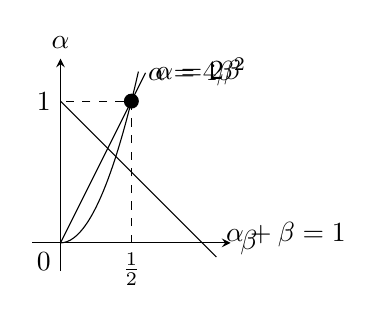
\begin{tikzpicture}[scale=1.8, >=stealth]
  \draw[->] (-0.2,0) -- (1.2,0) node[right] {$\beta$};
  \draw[->] (0,-0.2) -- (0,1.3) node[above] {$\alpha$};
  \node[below left] at (0,0) {$0$};
  
  \draw[domain=0:0.55, smooth, variable=\x] plot (\x, {4*\x*\x}) node[right] {$\alpha=4\beta^2$};
  \draw[domain=0:0.6, smooth, variable=\x] plot (\x, {2*\x}) node[right] {$\alpha=2\beta$};
  \draw[domain=0:1.1, smooth, variable=\x] plot (\x, {1 - \x}) node[above right] {$\alpha+\beta=1$};
  
  \draw[dashed] (0.5,0) node[below] {$\frac{1}{2}$} -- (0.5,1) -- (0,1) node[left] {$1$};
  \fill (0.5,1) circle (1.5pt);
\end{tikzpicture}
\end{center}

\section*{第3問}

[解] $\dfrac{1}{p} + \dfrac{1}{q} = 1, \, 0 < p, \, 0 < q \quad \dots \text{①}$

$f(x) = \dfrac{1}{p}x^p - x + \dfrac{1}{q}$ とおく。$f'(x) = x^{p-1} - 1$ である。①から $1 < p$ だから, 下表できる。

\begin{center}
\begin{array}{c|c|c|c|c}
x & 0 & \dots & 1 & \dots \\
\hline
f' & & - & 0 & + \\
\hline
f & & \searrow & 0 & \nearrow
\end{array}
\quad (\text{①から } f(1)=0)
\end{center}

したがって,
\[
\begin{cases}
x = 1 \text{ の時 } x = \dfrac{1}{p}x^p + \dfrac{1}{q} \\[10pt]
x \ne 1 \text{ 〃 } x < \dfrac{1}{p}x^p + \dfrac{1}{q}
\end{cases}
_{\mathbin{/\mkern-6mu/}}
\]

\section*{第4問}

[解] $f(x) = x^2+ax+b, \, g(x) = x^2+cx+d$ とおく。共通接線を $l : y = h(x)$ とすると,
\[
\begin{cases}
f(x) - h(x) = (x-p)^2 \\[5pt]
g(x) - h(x) = (x-q)^2
\end{cases}
\quad \dots \text{①}
\]
だから, 辺々引いて,
\[ f(x) - g(x) = (x-p)^2 - (x-q)^2 = (2x - p - q)(q - p) \]
となり, $y = f(x)$ と $y = g(x)$ の交点の $x$ 座標は $x = \dfrac{p+q}{2}$ である。

したがって, 求める面積 $S$ として ①から, $p < q$ の時
\[
\begin{aligned}
S &= \int_p^{\frac{p+q}{2}} (x-p)^2 dx + \int_{\frac{p+q}{2}}^q (x-q)^2 dx \\[10pt]
&= \frac{1}{12}(q-p)^3
\end{aligned}
\]
$q < p$ の時もかんがえて, $S = \dfrac{1}{12}|q-p|^3_{\mathbin{/\mkern-6mu/}}$

\section*{第5問}

[解] $e(\theta) = \cos\theta + i\sin\theta$ とおく。3数 $\alpha_1, \alpha_2, \alpha_3$ に対し :
\[ \alpha_k = r_k e(\theta_k) \quad (r_k, \theta_k \in \mathbb{R}) \]
とする。$(k=1, 2, 3)$ まず, $r_1=0$ とする。この時, $\alpha_1=0$。$\alpha_1 \ne \alpha_2, \, \alpha_1 \ne \alpha_3$ から, $r_2, r_3 > 0$ である。
題意から,
\[ \alpha_2 \alpha_3 = \alpha_1, \alpha_2, \alpha_3 \]
$\therefore \alpha_2 = 1 \text{ or } \alpha_3 = 1 \quad (\because \alpha_1=0, \, 0 < |\alpha_2| \le |\alpha_3|)$
となる。対称性から前者のみ考える。この時, 題意から,
\[ \alpha_3^2 = 0, 1, \alpha_3 \]
だが, $\alpha_1 \ne \alpha_3, \, \alpha_2 \ne \alpha_3, \, \alpha_3 \ne \alpha_1$ を満たすのは $\alpha_3 = -1$ のみである。以上から,
\[ (\alpha_1, \alpha_2, \alpha_3) = (0, 1, -1) \]
が必要である。この3数は条件を満たし, 十分である。 \dots ①

次に, $r_k > 0$ とする。この時, 題意から $r_k = 1$ が必要である。さらに, 題意から,
\[ \alpha_1 \alpha_2 = \alpha_1, \alpha_2, \alpha_3 \quad \dots (*) \]
となる。$\alpha_1 \alpha_2 = \alpha_1$ or $\alpha_1 \alpha_2 = \alpha_2$ の時 $\alpha_1 = 1$ or $\alpha_2 = 1$ となる。対称性から $\alpha_1 = 1$ とする。
この時, $\alpha_2 \ne 1, \, \alpha_3 \ne 1, \, \alpha_2 \ne \alpha_3$ より,
\[ \alpha_2 \alpha_3 = 1, \quad \alpha_2^2 = \alpha_3 \]
となり, $\{ \alpha_2, \alpha_3 \} = \left\{ e\left(\frac{2}{3}\pi\right), e\left(\frac{4}{3}\pi\right) \right\}$ をうる。逆にこの時, 十分である。 \dots ②

最後に, $(*)$ において $\alpha_1 \alpha_2 = \alpha_3$ の時, ①の場合をのぞいて, $\alpha_1 \ne 1, \alpha_2 \ne 1, \alpha_3 \ne 1$ と想定して良い。
この時同様に
\[
\begin{cases}
\alpha_2 \alpha_3 = \alpha_1 \\
\alpha_3 \alpha_1 = \alpha_2
\end{cases}
\quad \dots (**)
\]
をうるから, 辺々かけて, $\alpha_1 \alpha_2 \alpha_3 \ne 0$ から, 両辺 $\alpha_1 \alpha_2 \alpha_3$ でわって,
\[ \alpha_1 \alpha_2 \alpha_3 = 1 \]
$\alpha_1 \alpha_2 = \alpha_3$ から
\[ \alpha_3^2 = 1 \]
$\alpha_3 \ne 1$ から
\[ \alpha_3 = -1 \]
$(**)$ から $\alpha_2 = -\alpha_1$ となり, $\alpha_1 \alpha_2 = -\alpha_1^2 = -1$ とあわせて, $\alpha_1^2 = 1$ をうる。$\alpha_1 \ne 1, \alpha_3$ に反し矛盾。 \dots ③

以上①〜③より, もとめる3数は
\[ (0, 1, -1), \quad \left(1, -\frac{1}{2}+\frac{\sqrt{3}}{2}i, -\frac{1}{2}-\frac{\sqrt{3}}{2}i\right) _{\mathbin{/\mkern-6mu/}} \]

\section*{第6問}

[解] $C = \cos x, \, S = \sin x$ とおく。$I = \int_0^\pi x S e^x dx$ とおく。
\[
\begin{aligned}
I &= [x S e^x]_0^\pi - \int_0^\pi (S + x C) e^x dx = -\int_0^\pi S e^x dx - \int_0^\pi C x e^x dx \quad \dots \text{①} \\[5pt]
\int_0^\pi C x e^x dx &= [C x e^x]_0^\pi - \int_0^\pi (C - S x) e^x dx \\[5pt]
&= -\pi e^\pi - \int_0^\pi C e^x dx + I \quad \dots \text{②}
\end{aligned}
\]

$A = \int_0^\pi S e^x dx, \, B = \int_0^\pi C e^x dx$ とおく。①, ②に代入して
\[
\begin{aligned}
I &= -A + \pi e^\pi + B - I \\[5pt]
\therefore I &= \frac{\pi e^\pi + B - A}{2} \quad \dots \text{③}
\end{aligned}
\]

ここで,
\[
\begin{aligned}
A &= \frac{1}{1+1} [e^x(S-C)]_0^\pi = \frac{1}{2}(e^\pi + 1) \\[5pt]
B &= \frac{1}{1+1} [e^x(C+S)]_0^\pi = \frac{1}{2}(-e^\pi - 1)
\end{aligned}
\]

だから③に代入して
\[ I = \frac{\pi e^\pi - e^\pi - 1}{2} = \frac{(\pi-1)e^\pi - 1}{2} _{\mathbin{/\mkern-6mu/}} \]

[解2]
\[
\begin{aligned}
I &= [-C x e^x]_0^\pi + \int_0^\pi C e^x(x+1) dx = \pi e^\pi + B + \int_0^\pi C e^x x dx \\[5pt]
\int_0^\pi C e^x x dx &= [S e^x x]_0^\pi - \int_0^\pi S e^x (x+1) dx = -A - I
\end{aligned}
\]
だから
\[
\begin{aligned}
I &= \pi e^\pi + B - A - I \\[5pt]
\therefore I &= \frac{\pi e^\pi + B - A}{2}
\end{aligned}
\]
(以下略)

\end{document}
